\documentclass[usenames,dvipsnames]{beamer}
    \mode<presentation> {
    \usetheme{Montpellier}
    \usecolortheme{beaver}
    %\setbeamertemplate{footline} % To remove the footer line in all slides uncomment this line
    \setbeamertemplate{footline}[page number] % To replace the footer line in all slides with a simple slide count uncomment this line
    \setbeamertemplate{navigation symbols}{} % To remove the navigation symbols from the bottom of all slides uncomment this line
    }

    \usepackage{graphicx} % Allows including images
    \usepackage{booktabs} % Allows the use of \toprule, \midrule and \bottomrule in tables
    \usepackage[outputdir=target]{minted}
    \usepackage{xcolor}
    \usepackage[utf8]{inputenc}
    \usepackage{pifont}
    \usepackage{xspace}
    \usepackage{newunicodechar}
    \newunicodechar{✪}{\ding{74}}

    \definecolor{mintedbackground}{rgb}{0.95,0.95,0.95}
    \newcommand{\code}[1]{\colorbox{lightgray}{\texttt{#1}}}
    \newcommand{\distage}{\texttt{distage}\xspace}

\newminted{scala}{
    bgcolor=mintedbackground,
    fontfamily=tt,
    linenos=true,
    numberblanklines=true,
    numbersep=5pt,
    gobble=0,
    frame=leftline,
    framerule=0.4pt,
    framesep=2mm,
    funcnamehighlighting=true,
    tabsize=4,
    obeytabs=false,
    mathescape=false
    samepage=false, %with this setting you can force the list to appear on the same page
    showspaces=false,
    showtabs =false,
    texcl=false,
}

\newminted{text}{
    bgcolor=mintedbackground,
    fontfamily=tt,
    linenos=true,
    numberblanklines=true,
    numbersep=5pt,
    gobble=0,
    frame=leftline,
    framerule=0.4pt,
    framesep=2mm,
    funcnamehighlighting=true,
    tabsize=4,
    obeytabs=false,
    mathescape=false
    samepage=false, %with this setting you can force the list to appear on the same page
    showspaces=false,
    showtabs =false,
    texcl=false,
}

\newminted{json}{
    bgcolor=mintedbackground,
    fontfamily=tt,
    linenos=true,
    numberblanklines=true,
    numbersep=5pt,
    gobble=0,
    frame=leftline,
    framerule=0.4pt,
    framesep=2mm,
    funcnamehighlighting=true,
    tabsize=4,
    obeytabs=false,
    mathescape=false
    samepage=false, %with this setting you can force the list to appear on the same page
    showspaces=false,
    showtabs =false,
    texcl=false,
}

    \setminted{fontsize=\footnotesize,baselinestretch=1}

    \usepackage {tikz}
    \usetikzlibrary {positioning}
    \graphicspath {{target/media/}}

    \title[\distage]{\distage: Modern Staged Dependency Injection for Scala}

    \institute[Septimal Mind Ltd]
    {
    Septimal Mind Ltd\\
    \medskip
    \textit{team@7mind.io}
    }
    \date{\today}

\begin{document}

% \begin{VerbatimOut}{ex-scala-roles.tmp}
% @RoleId("testservice")
% class TestService[F[_] : Monad](http: HttpSrv[F])
%   extends IzService {
%     override def start(): Unit = http.start()
%     override def stop(): Unit = http.stop()
% }
% class TestPlugin extends PluginDef {
%   many[IzService].add[TestService[IO]]
% }
% object TestLauncher {
%   // run with
%   // java test.jar test-service other-service
%   def main(args: Array[String]): Unit = IzRoleApp(args).main()
% }
% \end{VerbatimOut}

\begin{frame}
%\titlepage
\begin{figure}
\Huge
\color{RubineRed} dist✪ge
\noindent
\rule{\linewidth}{1mm}
\Large Modern Staged Dependency Injection for Scala
\rule{\linewidth}{1mm}
\end{figure}

\begin{figure}
\color{RubineRed}
\normalsize Modular Functional Programming \\
with \\
Context Minimization \\
through \\
Garbage Collection
\end{figure}

\begin{figure}
\Large Septimal Mind Ltd \\
\medskip
\textit{team@7mind.io}
\end{figure}

\end{frame}

\section{The problem: Dependency Injection and Functional Programming}

\begin{frame}
\frametitle{The motivation behind DI pattern and DI frameworks}
\begin{enumerate}
\item Systems we work with may be represented as graphs. Nodes are components (usually instances), edges are references,
\item Graph transformation complexity grows non-linearly with node count (need to add one constructor parameter, have to modify $k$ classes),
\item Graph composition has combinatoric complexity (need to run tests choosing between mock/production repositories and external APIs, have to write four configurations).
\end{enumerate}

We have several possible options to address these problems:

\begin{enumerate}
\item Singletons and Factories: partially solve (2), code still tight coupled $\Rightarrow$ expensive tests and refactorings,
\item Service Locator: bit less coupled code, still very expensive,
\item Dependency Injection: less invasive, simplifies isolation but requires more complex machinery.
\end{enumerate}

\end{frame}

\begin{frame}
\frametitle{``DI doesn't compose with FP'': Problems}
\begin{enumerate}
\item Typical DI framework is OOP oriented and does not support advanced concepts required for modern FP (typeclasses, higher-kinded types),
\item Almost all the DI frameworks are working in runtime while many modern FP concepts are compile-time by their nature,
\item Less guarantees: program which compiles correctly can break on wiring in runtime. After a huge delay,
\item Wiring is non-determenistic: Guice can spend several minutes trying to re-instantiate heavy instance multiple times (once per dependency) then fail,
\item Wiring is opaque: it's hard or impossible to introspect the context. E.g. in Guice it's a real pain to close all the instantiated \texttt{Closeable}s.
      Adding missing values into the context (config injections) is not trivial as well.
\end{enumerate}
\end{frame}

\begin{frame}
\frametitle{``DI doesn't compose with FP'': Notes}
\begin{enumerate}
\item We have some compile-time DI frameworks or mechanisms (see \texttt{MacWire}) allowing us to implement DI as pattern
      though purely compile-time tools are not convenient when we have to deal with purely runtime entities
      (like plugins and config values),
\item Graph composition problem is not addressed by any existing tool.
\end{enumerate}
\end{frame}

\section{\distage: Staged DI for Scala}
\subsection{\distage: how it works}

\begin{frame}
\frametitle{DI implementations are broken\dots}
\dots so we may build better one, which must:
\begin{enumerate}
\item be well-integrated with type system of our target language (higher-kinded types, implicits, typeclasses),
\item allow us to introspect and modify our context on the fly,
\item be able to detect as many as possible problems quickly, better during compilation,
\item give us a way to stop making atomic or conditional contexts.
\end{enumerate}
\end{frame}

\begin{frame}
\frametitle{Staged approach}
\begin{enumerate}
\item Let's apply \textit{Late Binding},
\item let's collect our graph information first,
\item then build a DAG representing our context (so-called \textit{Project Network}, let's call it \textit{Plan}),
\item then analyse this graph for errors (missing references, conflicts),
\item then apply additional transformations,
\item then interpret the graph.
\end{enumerate}
This is a cornercase of more generic pattern -- PPER (Percept, Plan, Execute, Repeat).
\end{frame}

\begin{frame}
\frametitle{Staged approach: outcome}
What we get:
\begin{enumerate}
\item Planner is \textit{pure}: it has no side-effects,
\item A plan is a Turing-incomplete program for a simple machine. It will always terminate in known finite time,
\item An interpreter may perform instantiations at runtime or\dots just generate Scala code that will do that when compiled,
\item All the job except for instantiations can be done in compile-time,
\item Interpreter is free to run independent instantiations in parallel,
\item Extremely important: we can transform (rewrite) the plan before we run iterpreter.
\end{enumerate}
\end{frame}

\begin{frame}[fragile]
\begin{center}
\frametitle{Compile-Time and Runtime DI}
A Plan:
\begin{textcode}
myRepository := create[MyRepository]()
myservice    := create[MyService](myRepository)
\end{textcode}

May be interpreted as:

\begin{columns}

\begin{column}[T]{0.5\textwidth}
   \setlength{\topsep}{0pt}
   \setlength{\partopsep}{0pt}
Code tree (compile-time):
\begin{scalacode}
val myRepository =
    new MyRepository()
val myservice =
    new MyService(myRepository)
\end{scalacode}
\end{column}

\begin{column}[T]{0.5\textwidth}
Set of instances (runtime):
\begin{scalacode}
plan.foldLeft(Context.empty) {
case (ctx, op) =>
    ctx.withInstance(
        op.key
        , interpret(action)
    )
}
\end{scalacode}
\end{column}

\end{columns}
\end{center}
\end{frame}

\begin{frame}[fragile]
\frametitle{Incomplete plans}
This code:
\begin{scalacode}
class UsersRepoImpl(cassandraCluster: Cluster)
    extends UsersRepo
class UsersService(repository: UsersRepo)

class UsersModule extends ModuleDef {
  make[UsersRepo].from[UsersRepoImpl]
  make[UsersService]
}
\end{scalacode}

May produce a plan like:
\begin{textcode}
cassandraCluster     := import[Cluster]
usersRepo: UsersRepo := create[UsersRepoImpl](cassandraCluster)
usersService         := create[UsersService](usersRepo)
\end{textcode}
\end{frame}

\subsection{patterns and Extensions}
\begin{frame}
\begin{figure}
\Huge
\color{RubineRed} dist✪ge
\noindent
\rule{\linewidth}{1mm}
\Large Patterns and Extensions
\rule{\linewidth}{1mm}
\end{figure}
\end{frame}

\begin{frame}[fragile]
\frametitle{Pattern: Plan completion}
Once we have such a plan:
\begin{textcode}
cassandraCluster     := import[Cluster]
usersRepo: UsersRepo := create[UsersRepoImpl](cassandraCluster)
usersService         := create[UsersService](usersRepo)
\end{textcode}

We may add missing values\footnotemark[1]:

\begin{scalacode}
val plan = Injector.plan(definitions)
val resolved = plan.map {
  case i: Import if i.is[Cluster] =>
    val cluster: Cluster = ???
    Reference(cluster)
  case op => op
}
\end{scalacode}
\footnotetext[1]{Pseudocode, real API is bit different}
\end{frame}


\begin{frame}[fragile]
\frametitle{Extension: Configuration Support}

\distage has \texttt{HOCON} configuration support implemented as an extension.

\begin{scalacode}
case class HostPort(host: String, port: Int)

class HttpServer(@ConfPath("http.listen") listenOn: HostPort) {
  // ...
}
\end{scalacode}

The extension:
\begin{enumerate}
\item Takes all the Imports of a Plan,
\item Searches them for a specific \mintinline{scala}{@ConfPath} annotation,
\item Tries to find corresponding sections in config,
\item Extends plan with config values,
\end{enumerate}
All the config values are resolved even before instantiation of services $\Rightarrow$ problems are being shown quickly and all at once.
\end{frame}

\begin{frame}[fragile]
\frametitle{Extension: Automatic Sets}

\begin{enumerate}
\item \distage can find all instances type \mintinline{scala}{T} (like \mintinline{scala}{AutoCloseable}) in the context,
put them all into a \mintinline{scala}{Set[T]} then inject that set.
\item $\Rightarrow$ basic lifecycle support, free of charge.
\end{enumerate}

\begin{scalacode}
trait Resource {
  def start(): Unit
  def stop(): Unit
}
trait App { def main(): Unit }
locator.run { (resources: Set[Resource], app: App) =>
  try {
    resources.foreach(_.start())
    app.main()
  } finally {
    resources.foreach(_.close())
  }
}
\end{scalacode}
\end{frame}

\begin{frame}
\frametitle{The Principle Behind: Feedback Loops}
They use so-called \textit{Feedback Loops} in robotics\dots
\begin{figure}
    
\includegraphics[width=0.8\textwidth]{media/robots.jpg}
\end{figure}
\end{frame}

\begin{frame}
    \frametitle{The Principle Behind: PPER Loop\footnotemark[1]}

    We found a very generic and important pattern of \textit{Feedback Loop} class:
\begin{enumerate}
    \item Acquire data from the outer world (\textit{Percept})
    \item Produce a Project Network, \textit{Plan}.
          It may be incomplete, but should allow us to progress (\textit{Plan})
          \begin{itemize}
            \item Plan is a DAG, actions are nodes, edges are dependencies
          \end{itemize}
    \item Execute the Plan (\textit{Execute}).
    \begin{itemize}
        \item Perform the steps of the Plan
        \item Mark your Plan nodes according to the results of their execution
        \item Let's call marked plan as \textit{Trace}
      \end{itemize}
    \item Go to step 1 unless termination criteria reached (\textit{Repeat})
\end{enumerate}
Let's call it \textit{PPER} (pronounced: \textit{pepper}).
\footnotetext[1]{Slides: https://goo.gl/okZ8Bw}
\end{frame}

\subsection{Garbage Collector and its Benefits}

\begin{frame}
\frametitle{Garbage Collector and Context Minimization}
\begin{enumerate}
\item Let's assume that we have a \mintinline{scala}{UsersService} and \mintinline{scala}{AccountingService}
      in your context,
\item \dots and we want to write a test for \mintinline{scala}{UsersService} only,
\item We may exploit staged design and \textit{collect the garbage} out of Plan before executing it.
\item We define a \textit{garbage collection root}, \mintinline{scala}{UsersService}, and keep only
the operations it transitively depends on. The rest is being thrown out \textbf{even before it's being instantiated},
\item Garbage Collector allows us to compose contexts easier.
\end{enumerate}
\end{frame}

\begin{frame}
\frametitle{Garbage Collector and Context Minimization}
\begin{figure}
    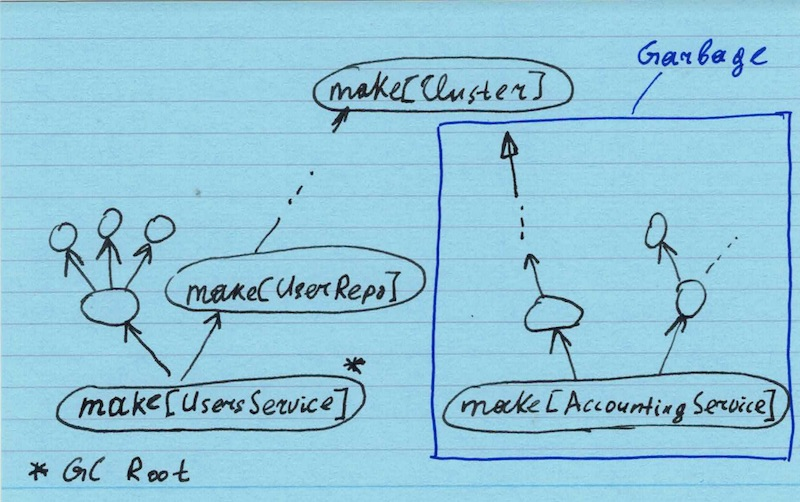
\includegraphics[width=\textwidth]{media/gc-ex.jpg}
\end{figure}
\end{frame}

\begin{frame}
\frametitle{Context Minimization for Tests}
Context minimization allows us to:
\begin{enumerate}
\item Instantiate only the instances which are required for your tests,
\item Save on test startup time (savings may be significant),
\item Save on configuring per-test contexts manually (savings may be substantial).
\end{enumerate}
\end{frame}

\begin{frame}[fragile]
\frametitle{Context Minimization for Deployment}
Context minimization allows us to:
\begin{enumerate}
\item Have one image with all our software components (\textit{Roles}\footnotemark[1]),
\item \dots keeping development flows of these components isolated,
\item Decide which components we want to run when we start the image,
\item Have higher computational density
\item \textit{substantially} simplify development flows: we may run full environment with a single command on a low-end machine,
\item Fuse Microservices with Monoliths keeping \textit{all} their benefits.
\end{enumerate}

\begin{textcode}
server1# docker run -ti company/product +analytics
server2# docker run -ti company/product +accounting +users
laptop# docker run -ti company/product --run-everything
\end{textcode}

\footnotetext[1]{Slides: https://goo.gl/iaMt43}
\end{frame}

\subsection{Scala Typesystem Integration: Fusional Programming}
\begin{frame}
\begin{figure}
\Huge
\color{RubineRed} dist✪ge
\noindent
\rule{\linewidth}{1mm}
\Large Scala Typesystem Integration:\\
Fusional Programming
\rule{\linewidth}{1mm}
\end{figure}
\end{frame}


\begin{frame}[fragile]
\frametitle{Kind-Polymorphic Type Tags}
\begin{columns}

\begin{column}[T]{0.4\textwidth}
   \setlength{\topsep}{0pt}
   \setlength{\partopsep}{0pt}
\begin{itemize}
\item \distage uses types as lookup keys
\item But \texttt{scalac} has \texttt{TypeTags} only for kind \texttt{*}!
\item \distage added any-kinded `Tag`s
\item Modules can be polymorphic on types of any kind
\end{itemize}
\end{column}

\begin{column}[T]{0.6\textwidth}
\begin{scalacode}
def m1[F[_]: TagK: Monad, A: Encoder]
  = new ModuleDef {
      addImplicit[Encoder[A]]
      make[SendJson[F, A]]
    }
// `Tag` implicit accepts
// type parameters of any kind
def meta[FT[_[_], _]: Tag.auto.T] =
  new ModuleDef {
    make[FT[IO, Int]]
  }
\end{scalacode}
\end{column}

\end{columns}
\begin{scalacode}
type TagK[F[_]] = HKTag[{ type Arg[A] = F[A] }]
type TagKK[F[_, _]] = HKTag[{ type Arg[A, B] = F[A, B] }]
\end{scalacode}
\footnotetext[1]{Tag.auto.T macro will be added in next version}
\end{frame}

\begin{frame}[fragile]
\frametitle{Typeclass instance injection (Implicit Injection)}
\begin{enumerate}
\item \distage wires \textit{all} parameters, inlcuding implicits
\item Leaving implicits solely to implicit resolution would've been \textit{unmodular},
because we want to bind instances \textit{late}, not at definition time
\item Therefore implicits should be declared explicitly
\item Tagless-final style is encouraged – add implicit parameters, instead of importing concrete implicits!
\begin{scalacode}
def polyModule[F[_]: Sync: TagK] = new ModuleDef {
  make[Sync[F]].from(implicitly[Sync[F]])
  make[F[Unit]].named("hello").from(
    S: Sync[F] => S.delay(println("Hello World!")))
}
Injector()
  .produce(polyModule[cats.effect.IO])
  .get[IO[Unit]]("hello").unsafeRunSync()
\end{scalacode}
\end{enumerate}
\end{frame}

\begin{frame}[fragile]
\frametitle{Lambda Injection, ProviderMagnet}
\begin{enumerate}
\item We can bind functions as constructors
\item Arbitrary-arity functions can run with arguments from Locator
\item Put annotations on types to summon named instances or config values (from \texttt{distage-config})
\end{enumerate}
\begin{scalacode}
case class A()
case class B(a: A)
val ctx: Locator = Injector(config).produce(new ModuleDef {
  make[A].from(() => A())
  make[B].from(B(_))
})
case class C(a: A, b: B, host: HostPort)
val c: C = ctx.run {
  (a: A, b: B, host: HostPort @ConfPath("http.listen")) =>
    C(a, b, host)
}
\end{scalacode}
\end{frame}

\begin{frame}[fragile]
\frametitle{Code example: IO Injection}
\begin{enumerate}
\begin{scalacode}
trait MonadFilesystem[F[_, _]] {
  def readFile(fileName: String): F[Exception, String]
}

class ZioFilesystemModule extends ModuleDef {
  make[MonadFilesystem[IO]].from(new MonadFilesystem[IO] {
    def readFile(fileName: String) =
      IO.syncException(Source.fromFile(fileName)("UTF-8")
        .mkString)
  })
}

class GetCpusModule extends ModuleDef {
  make[IO[Exception, Int]].named("getCpus").from {
    fs: MonadFilesystem[IO] =>
      fs.readFile("/proc/cpuinfo").flatMap(...)
  }
}
\end{scalacode}
\end{enumerate}
\end{frame}

\begin{frame}[fragile]
\frametitle{Code example: Tagless Final Style}
\begin{enumerate}

\begin{scalacode}
trait Interaction[F[_]] {
  def say(msg: String): F[Unit]
  def ask(prompt: String): F[String]
}

class TaglessHelloWorld[F[_]: Monad: Interaction] {
  def program = for {
      userName <- Interaction[F].ask("What's your name?")
      _        <- Interaction[F].say(s"Hello $userName!")
  } yield ()
}

val wiring = new ModuleDef {
  make[TaglessHelloWorld[Try]]
  make[Interaction[Try]].from(new Interaction[Try] {...})
}
\end{scalacode}

\end{enumerate}
\end{frame}

\begin{frame}[fragile]
\frametitle{Path-dependent types}
\begin{enumerate}
\item Path-dependent types and projections are supported
\item Path-prefix should be wired for the child type to be wired
\end{enumerate}
\begin{scalacode}
trait Cake { trait Child }

val cakeModule = new ModuleDef {
  make[Cake]
  make[Cake#Child]
}
val cake = Injector().produce(cakeModule).get[Cake]

val instanceCakeModule = new ModuleDef {
  make[cake.type].from[cake.type](cake: cake.type)
  make[cake.Child]
}
val cakeChild = Injector().produce(instanceCakeModule)
  .get[cake.Child]
\end{scalacode}
\end{frame}

\subsection{Features to boost productivity}
\begin{frame}
\begin{figure}
\Huge
\color{RubineRed} dist✪ge
\noindent
\rule{\linewidth}{1mm}
\Large Features to boost productivity
\rule{\linewidth}{1mm}
\end{figure}
\end{frame}

\begin{frame}[fragile]
\frametitle{Dynamic Plugins}
Just drop your modules into your classpath:
\begin{scalacode}
class AccountingModule extends PluginDef {
  make[AccountingService].from[AccountingServiceImpl]
  // ...
}
\end{scalacode}
Then you may pick up all the modules and build your context:
\begin{scalacode}
val plugins = new PluginLoaderDefaultImpl(
  PluginConfig(Seq("com.company.plugins"))
).load()
// ... pass to an Injector
\end{scalacode}
\begin{enumerate}
\item Useful while you are prototyping your app,
\item In maintenance phase you may switch to static configuration.
\end{enumerate}
\end{frame}

\begin{frame}[fragile]
\frametitle{Dynamic Testkit (ScalaTest)}
\begin{scalacode}
class AccountingServiceTest extends DistagePluginSpec {
  "accounting service" must {
    "be resolved dynamically" in di {
      (acc: AccountingService) =>
        assert(acc.getBalance("bad-user") == 0)
    }
  }
}
\end{scalacode}

\begin{enumerate}
\item You don't need to setup your context, it's done automatically by Plugin Loader and Garbage Collector,
\item And it takes just milliseconds, not like in Spring,
\item Garbage collection roots are inferred from test's signature,
\item Only the things required for a particular test are being instantiated.
\end{enumerate}
\end{frame}

\begin{frame}[fragile]
\frametitle{Tags}
\begin{enumerate}
\item Each binding may be marked with a \textit{tag},
\item Some bindings may be excluded from the context before planning by a predicate,
\item This is unsafe but convenient way to reconfigure contexts conditionally.
\end{enumerate}

\begin{scalacode}
class ProductionPlugin extends PluginDef {
  tag("production", "cassandra")
  make[UserRepo].from[CassandraUserRepo]
}
class MockPlugin extends PluginDef {
  tag("test", "mock")
  make[UserRepo].from[MockUserRepo]
}
// ...
val disabledTags = t"mock" && t"dummy"
val plan = injector.plan(definition.filter(disabledTags))
\end{scalacode}

\end{frame}

\begin{frame}
\frametitle{Circular dependencies}
\begin{enumerate}
\item Supported, \texttt{Proxy} concept used,
\item By-name parameters (\mintinline{scala}{class C(param: => P)}) supported, no runtime code-generation requried,
\item Other cases are supported as well with runtime code-generation,
\item Limitations: typical. You cannot use an injected parameter immediately in a constructor,
   you cannot have circular non-by-name dependencies with final classes,
\item Circular dependency resolution is optional, you may turn it off.
\end{enumerate}
\end{frame}

\begin{frame}[fragile]
\frametitle{Plan Introspection: example context}
\begin{scalacode}
class Cluster
trait UsersService
trait AccountingService
trait UserRepo
trait AccountsRepo

class UserRepoImpl(cluster: Cluster) extends UserRepo
class AccountsRepoImpl(cluster: Cluster) extends AccountsRepo
class UserServiceImpl(userRepo: UserRepo) extends UsersService
class AccountingServiceImpl(accountsRepo: AccountsRepo)
    extends AccountingService

class UsersApiImpl(service: UsersService
    , accountsApi: AccountsApiImpl)
class AccountsApiImpl(service: AccountingService
    , usersApi: UsersApiImpl) // circular dependency
class App(uapi: UsersApiImpl, aapi: AccountsApiImpl)
\end{scalacode}
\end{frame}

\begin{frame}[fragile]
\frametitle{Plan Introspection: example bindings\footnotemark[1]}
\begin{scalacode}
val definition = new ModuleDef {
    make[Cluster]
    make[UserRepo].from[UserRepoImpl]
    make[AccountsRepo].from[AccountsRepoImpl]
    make[UsersService].from[UserServiceImpl]
    make[AccountingService].from[AccountingServiceImpl]
    make[UsersApiImpl]
    make[AccountsApiImpl]
    make[App]
}
val injector = Injector()
val plan = injector.plan(definition)
\end{scalacode}
\footnotetext[1]{Full code example: https://goo.gl/7ZwHfX}
\end{frame}

\begin{frame}[fragile]
\frametitle{Plan Introspection: plan dumps}
\begin{scalacode}
println(plan.render) // look for the circular dependency!
\end{scalacode}

\begin{figure}
    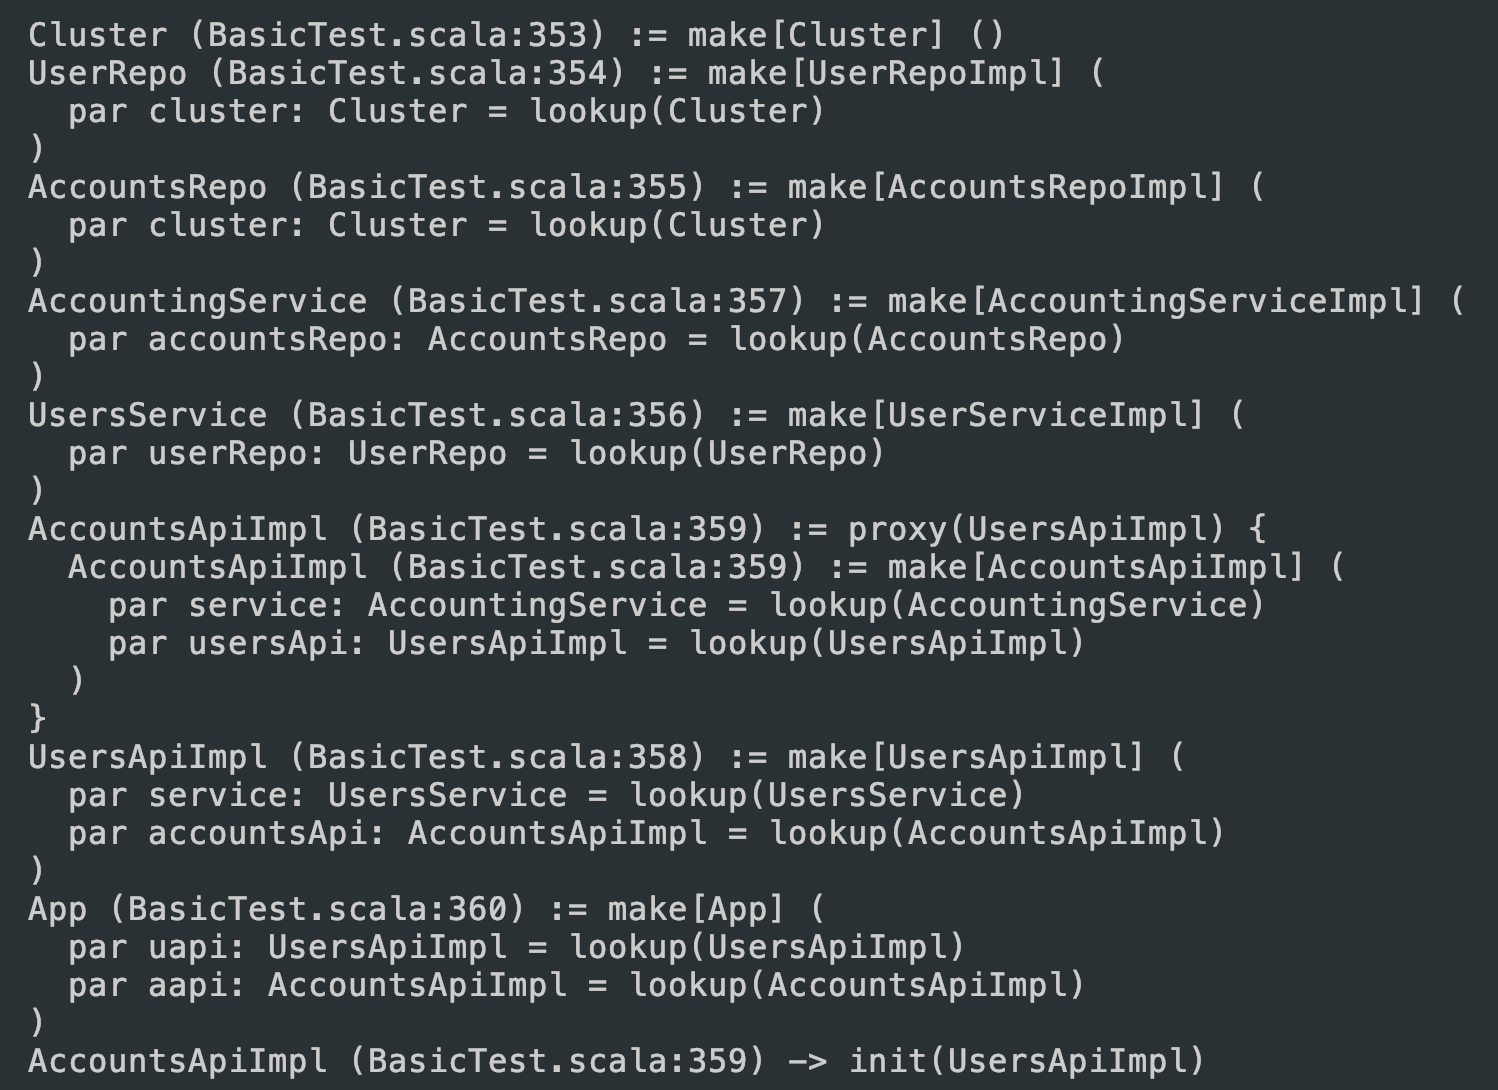
\includegraphics[width=0.75\textwidth]{media/plan-example.png}
\end{figure}
\end{frame}

\begin{frame}[fragile]
\frametitle{Plan Introspection: dependency trees}
You may explore dependencies of a component:

\begin{scalacode}
val dependencies = plan.topology.dependencies
println(dependencies.tree(DIKey.get[AccountsApiImpl]))
\end{scalacode}

\begin{figure}
    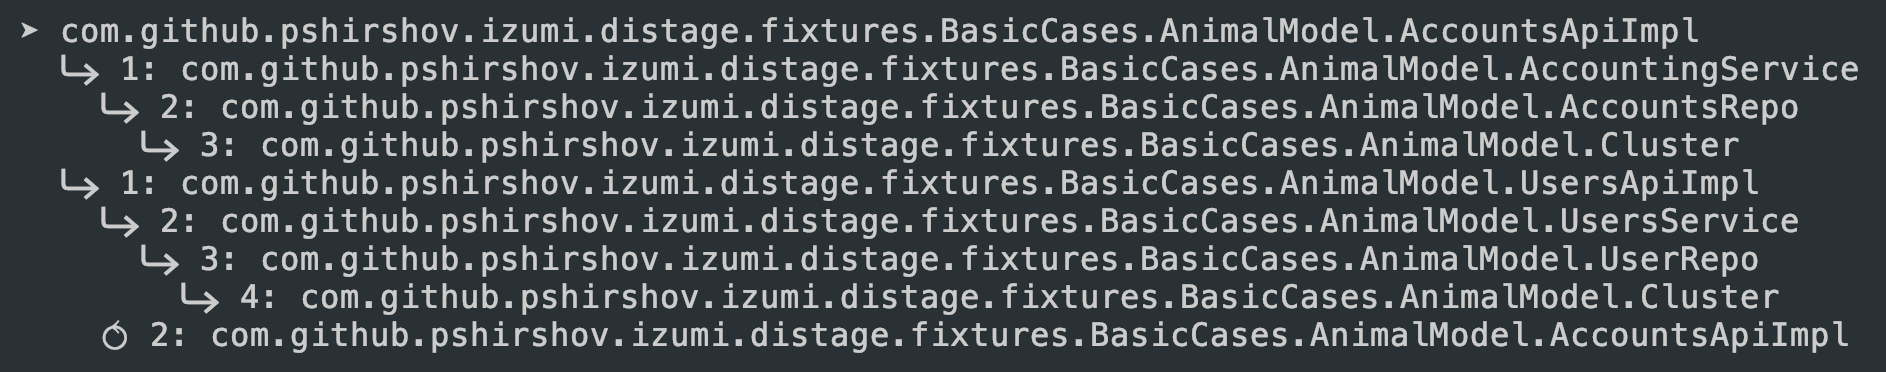
\includegraphics[width=\textwidth]{media/dependency-tree.png}
\end{figure}

Circular dependencies are specifically marked.
\end{frame}

\begin{frame}[fragile]
\frametitle{Trait Completion}
\begin{scalacode}
trait UsersService {
  protected def repository: UsersRepo
  def add(user: User): Unit = {
    repository.put(user.id, user)
    ???
  }
}
\end{scalacode}
We may bind this trait directly, without an implementation class:

\begin{scalacode}
make[UsersService]
\end{scalacode}

\begin{enumerate}
\item Corresponding class will be generated by \distage,
\item Null-arg abstract methods will be wired with context values,
\item Works in both runtime and compile-time.
\end{enumerate}
\end{frame}

\begin{frame}[fragile]
\frametitle{Factory Methods (Assisted Injection)}
\begin{scalacode}
class UserActor(sessionId: UUID, sessionRepo: SessionRepo)

trait ActorFactory {
  def createActor(sessionId: UUID): UserActor
}
\end{scalacode}

\begin{enumerate}
\item \mintinline{scala}{createActor} is a factory method,
\item \mintinline{scala}{createActor} will be generated by \distage,
\item non-null-arg abstract methods are treated as factory methods,
\item Non-invasive \textit{assisted injection}: \mintinline{scala}{sessionId: UUID} will be taken from method parameter, \mintinline{scala}{sessionRepo: SessionRepo} will be wired from context,
\item Useful for \texttt{Akka}, lot more convenient than Guice,
\item Works in both runtime and compile-time.
\end{enumerate}
\end{frame}


\subsection{7mind Stack}
\begin{frame}
\begin{figure}
\Huge
\color{RubineRed} dist✪ge
\noindent
\rule{\linewidth}{1mm}
\Large 7mind Stack
\rule{\linewidth}{1mm}
\end{figure}
\end{frame}

\begin{frame}
\frametitle{\distage: status and things to do}
\distage is:
\begin{enumerate}
\item ready to use,
\item in real production,
\item all Runtime APIs are available,
\item Compile-time verification, trait completion, assisted injections and lambda injections are available.
\end{enumerate}
\vspace{0.3cm}
Our plans:
\begin{enumerate}
\item Refactor Roles API,
\item Support running Producer within a monad (to use with \texttt{Scalaz ZIO}, \texttt{Monix}, \texttt{cats-effect}, etc),
\item Support Scala.js,
\item Support optional isolated classloaders (in foreseeable future),
\item Publish compile-time Producer,
\item Check our GitHub: https://github.com/pshirshov/izumi-r2.
\end{enumerate}
\end{frame}

\begin{frame}
\frametitle{\distage is just a part of our stack}
We have a vision backed by our tools:
\begin{enumerate}
\item Idealingua: transport and codec agnostic gRPC alternative with rich modeling language,
\item LogStage: zero-cost logging framework,
\item \textit{Fusional Programming and Design} guidelines. We love both FP and OOP,
\item \textit{Continous Delivery} guidelines for Role-based process,
\item \textit{Percept-Plan-Execute} Generative Programming approach, abstract machine and computational model.
Addresses Project Planning (see Operations Research). Examples: orchestration, build systems.
    %  Roles: distributed development without distributed computing

\end{enumerate}

Altogether these things already allowed us to significantly reduce development costs and
delivery time for our client.\newline

More slides to follow.
\end{frame}

\begin{frame}
\begin{center}
\Huge
You use \texttt{Guice}?

Switch to \distage!

\begin{figure}
    
\includegraphics[width=0.35\textwidth]{media/haruhi.jpg}
\end{figure}

\end{center}
\end{frame}

\begin{frame}[fragile]
\frametitle{Teaser: LogStage}
A log call \dots
\begin{scalacode}
log.info(s"$user logged in with $sessionId!")
\end{scalacode}

\dots may be rendered as a text like \texttt{17:05:18 UserService.login user=John Doe logged in with sessionId=DEADBEEF!}

\dots or a structured JSON:
\begin{jsoncode}
{
  "user": "John Doe",
  "sessionId": "DEADBEEF",
  "_template": "$user logged in with $sessionId!",
  "_location": "UserService.scala:265",
  "_context": "UserService.login",
}
\end{jsoncode}
\end{frame}

\begin{frame}[fragile]
\frametitle{Teaser: Idealingua}
\begin{textcode}
id UserId { uid: str }
data User {  name: str /* ... more fields */ }
data PublicUser {
 + InternalUser
 - SecurityAttributes
}
adt Failure = NotFound | UnknownFailure
service Service {
  def getUser(id: UserId): User !! Failure
}
\end{textcode}

\begin{enumerate}
\item Convenient Data and Interface Definition Language,
\item Extensible, transport-agnostic, abstracted from wire format,
% \item Server-to-Server, Server-to-Client \& Client-to-Server communication,
% \item Bifunctor Error Model, Strongly typed API calls - no longer remove type safety with microservices!
% \item <IMG>twitter microservices are a great way to remove typesafety</IMG>
\item JSON + HTTP / WebSocket at the moment,
\item C\#, go, Scala, TypeScript at the moment,
\item Better than gRPC/ REST / Swagger/ etc.
\end{enumerate}
\end{frame}

\begin{frame}
    \frametitle{Thank you for your attention}

    \begin{center}
      https://izumi.7mind.io/

      We're looking for clients, contributors, adopters and colleagues ;)
    \end{center}

    About the author:
    \begin{enumerate}
        \item coding for 18 years, 10 years of hands-on commercial engineering experience,
        \item has been leading a cluster orchestration team in Yandex, ``the Russian Google'',
        \item implemented ``\textit{Interstellar Spaceship}'' -- an orchestration solution to manage 50K+ physical machines across 6 datacenters,
        \item Owns an Irish R\&D company, https://7mind.io,
        \item Contact: team@7mind.io,
        \item Github: https://github.com/pshirshov
    \end{enumerate}
\end{frame}

\end{document}
